\documentclass[12pt,a4paper]{article}

\renewcommand*\contentsname{Sadržaj}
\renewcommand{\figurename}{Slika}

\usepackage[margin=0.85in]{geometry}
\usepackage{graphicx}
\usepackage{float}
\usepackage{listings}


% DODANO:
\renewcommand{\arraystretch}{1.5}
\begin{document}

\begin{titlepage}
	\centering
	{\scshape Univerzitet u Sarajevu \par}
	{\scshape Elektrotehnički Fakultet \par}
	\vspace{1cm}
	{\Large\scshape Prepoznavanje Oblika i Obrada Slike\par}
	\vspace{1.5cm}
	{\huge\bfseries Projektni Zadatak br. 2\par}
	\vspace{2cm}
	\Large Studenti: \par
	{\Large\itshape \textsc{Muftić} Belma, 1423/17260\par}
	{\Large\itshape \textsc{Lemeš} Lamija, 1474/17070\par}
	{\Large\itshape \textsc{Krupalija} Ehlimana, 1431/17461\par}
	\vfill
	Odgovorni asistent:\par
	MoE \textsc{Sumejja Porča}
	\vfill
	{\large December, 2018\par}
\end{titlepage}

\pagenumbering{gobble}

\tableofcontents

\newpage

\pagenumbering{arabic}
\setcounter{page}{1}

\section{Izbor modela za prepoznavanje}

Postoji šest najčešće korištenih klasifikacijskih modela (što je prikazano na Slici 1.):

\begin{enumerate}

\item SGD (\textit{Stohastic Gradient Descent}) klasifikacija;
\item \textit{Kernel Approximation} klasifikacija;
\item Linearna SVC (\textit{Support Vector Classification});
\item SVC (\textit{Support Vector Classification});
\item KNN (\textit{K-Nearest Neighbors}) klasifikacija;
\item \textit{Naive Bayes} klasifikacija.

\end{enumerate}

\begin{figure}[H]

\center
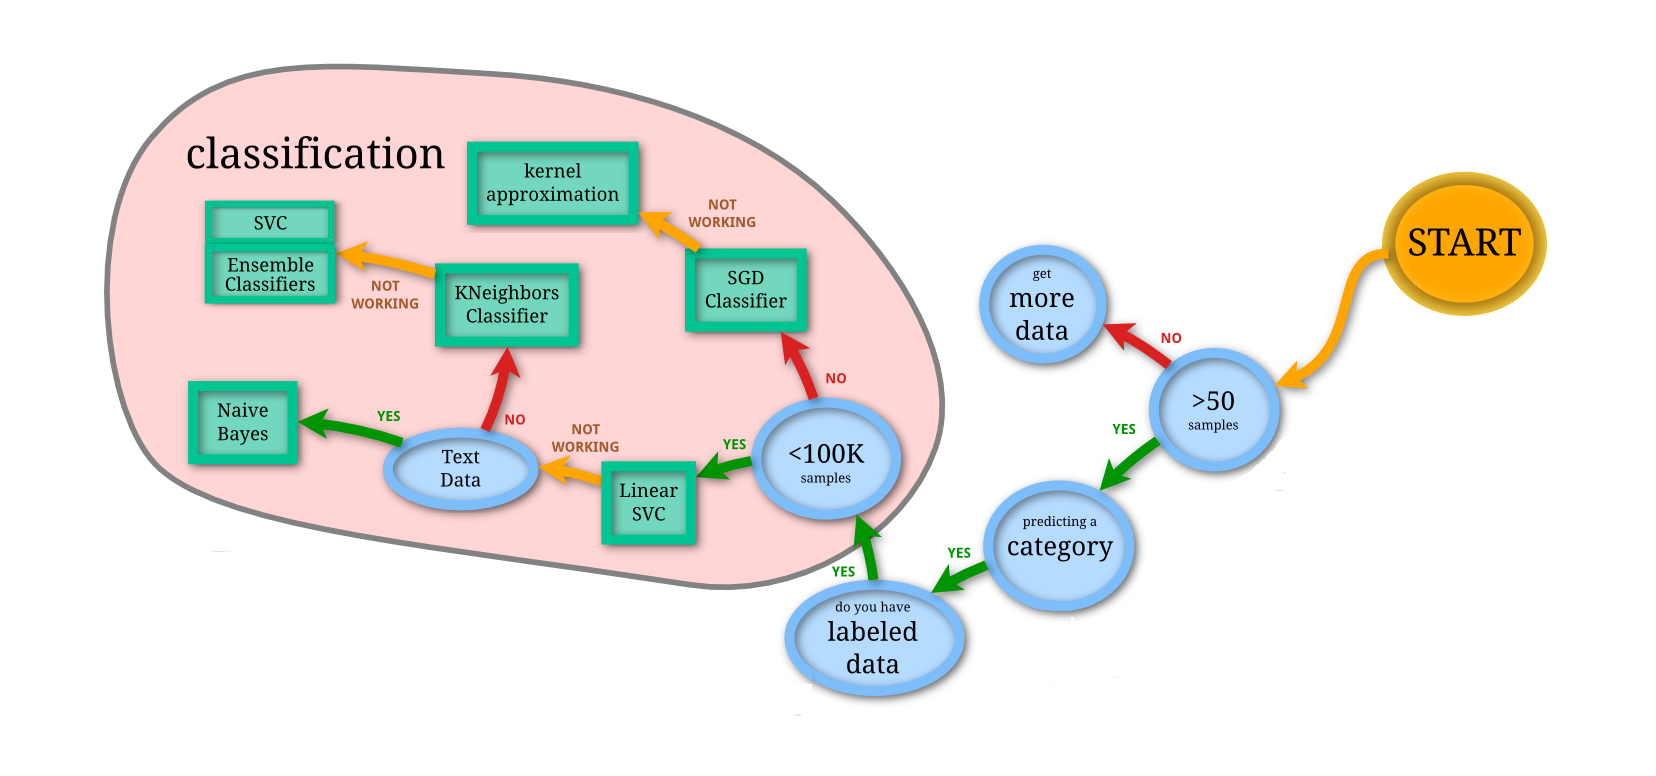
\includegraphics[scale=0.35]{slikaModeli.png}
\caption{Klasifikacijski modeli i vršenje njihovog odabira}
	
\end{figure}

Budući da \textit{dataset} ima manje od 100,000 slika, te postoje tekstualni podaci o različitim kategorijama i ROI, koristiti će se \textbf{\textit{Naive Bayes}} klasifikacijski model.

\newpage

\section{Izbor deskriptora}



\newpage

\section{Izbor metoda poboljšanja}

\subsection{Poboljšavanje kontrasta}

Od tri implementirane metode, najbolje rezultate pokazala je metoda \textbf{linearnog razvlačenja kontrasta}. Metoda aritmetičkih operacija previše je narušila strukturu slike, dok metoda \textit{gamma} korekcije nije izvršila dovoljnu modifikaciju kontrasta. Iz ovog razloga metoda linearnog razvlačenja kontrasta koristiti će se za poboljšavanje slika prije njihove dalje obrade.

\begin{figure}[H]

\center
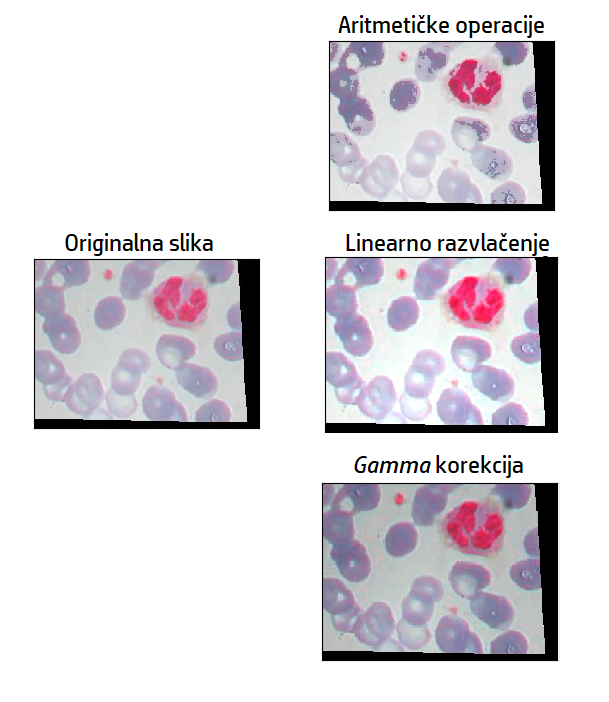
\includegraphics[scale=0.9]{slikaKontrast.png}
\caption{Rezultati korištenja različitih metoda za poboljšavanje kontrasta}
	
\end{figure}

\newpage

\subsection{Poboljšavanje osvjetljenja}

Od tri implementirane metode, najbolje rezultate pokazala je metoda \textbf{linearnih transformacija}. Metoda aritmetičkih operacija nije izvršila dovoljnu promjenu osvjetljenja, dok je metoda manipulacije HSV slikom izvršile preveliko povećanje osvjetljenja, te će se iz ovog razloga metoda linearnih transformacija koristiti za poboljšavanje slika prije njihove dalje obrade.

\begin{figure}[H]

\center
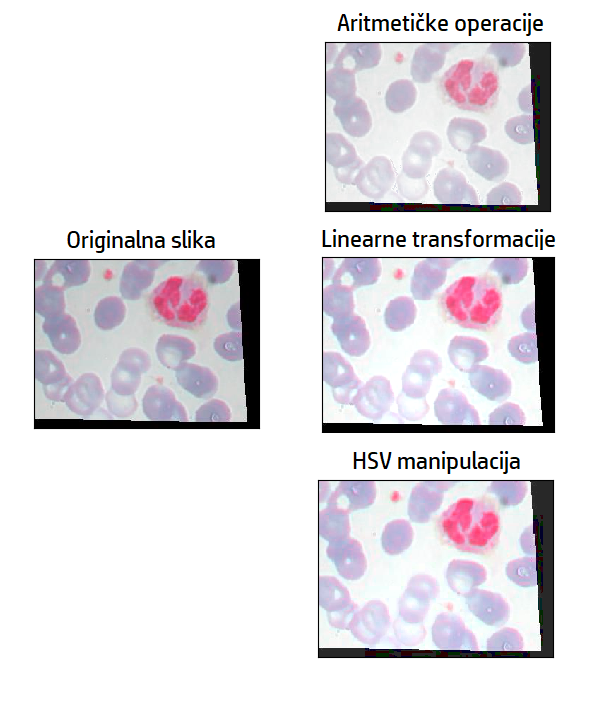
\includegraphics[scale=0.9]{slikaOsvjetljenje.png}
\caption{Rezultati korištenja različitih metoda za poboljšavanje osvjetljenja}
	
\end{figure}

\newpage

\subsection{Ujednačavanje histograma}

Od tri implementirane metode, najbolje rezultate pokazala je metoda \textbf{CLAHE}. Metoda raspodjele vjerovatnoća previše je degradirala strukturu slike (pri čemu su neke ćelije potpuno nestale sa slike, što je nedopustivo), dok je metoda \texttt{equalizeHist} degradirala strukturu slike u pogledu boje. Iz ovog razloga metoda CLAHE koristiti će se za poboljšavanje slika prije njihove dalje obrade.

\begin{figure}[H]

\center
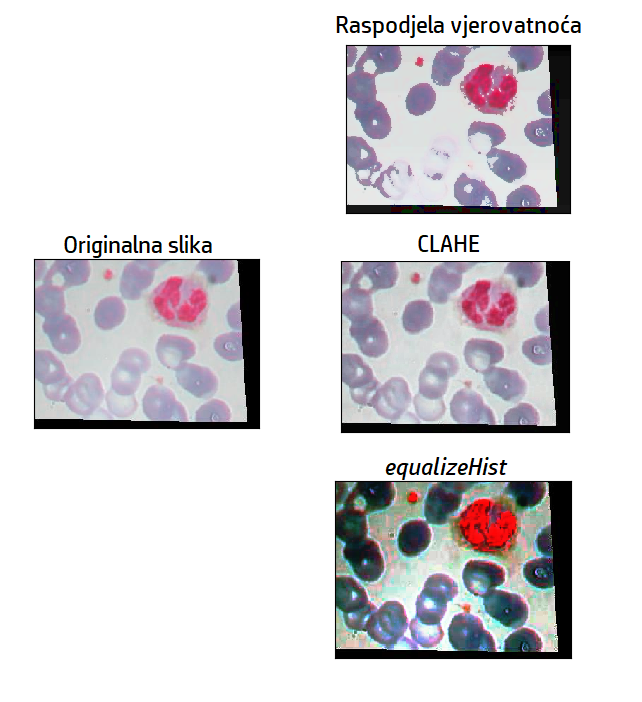
\includegraphics[scale=0.9]{slikaHistogram.png}
\caption{Rezultati korištenja različitih metoda za ujednačavanje histograma}
	
\end{figure}

\end{document}